\subsection{Casos de uso.}
En este apartado se describen los casos de uso del único actor que tiene el juego: el jugador. En la imagen \ref{fig:casosUso} se puede ver el diagrama de caso de uso del jugador.

\begin{figure}
	\centering
	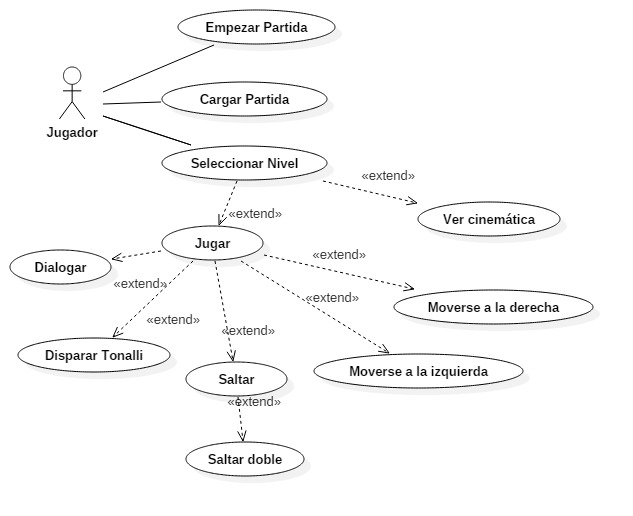
\includegraphics[width=\textwidth]{05TrabajoRealizado/01DocDiseno/imagenes/casoUso1.jpg}
	\caption{Caso de uso Jugador.}
	\label{fig:casosUso}
\end{figure}

\subsubsection{CU-001 Empezar partida.} \label{CU:01}
\begin{longtable}[c]{ | m{5cm} | m{10cm}|} 
		\hline
		\rowcolor{cyan}CU-001. & Empezar partida. \\ 
		\hline
		Descripción. & El jugador iniciará una nueva partida. \\ 
		\hline
		Reglas de negocio. & RN-00\ref{RN:01}\\ 
		\hline
		Precondición. & Existirá un archivo con los datos del juego en caso de que no sea la primera vez que se empiece una partida. \\
		\hline
		Postcondición. & Se generará un archivo con los datos de la partida.\\
		\hline
		Errores. & ER-001.\\
		\hline
\end{longtable}
\begin{itemize}
	\item[•] Trayectoria Principal.
		\begin{enumerate}
			\item El jugador inicia la aplicación.
			\item El jugador toca la pantalla táctil en la pantalla de inicio.
			\item El juego carga la interfaz del menú principal.
			\item El jugador selecciona el botón de Empezar partida (Ruta A).
			\item El juego despliega el mensaje 01 (Ruta B).
			\item El jugador pulsa selecciona el botón de aceptar, con lo que confirma la acción de empezar partida.
			\item El juego crea un archivo con los datos de la nueva partida.
		\end{enumerate}
	\item[•] Trayectorias Secundarias.
		\begin{itemize}
			\item Ruta A. 
				\begin{enumerate}
					\item El jugador selecciona el botón de Cargar partida (Ver caso de uso \ref{CU:02}).
				\end{enumerate}
			\item Ruta B.
				\begin{enumerate}
					\item El jugador selecciona el botón de cancelar.
					\item El jugador se queda en la interfaz del menú principal.
				\end{enumerate}
		\end{itemize}
\end{itemize}

\subsubsection{CU-002 Cargar partida.} \label{CU:02}
\begin{longtable}[c]{ | m{5cm} | m{10cm}|} 
		\hline
		\rowcolor{cyan}CU-002. & Cargar partida. \\ 
		\hline
		Descripción. & El jugador cargará una partida ya existente. \\ 
		\hline
		Reglas de negocio. & RN-00\ref{RN:01}\\ 
		\hline
		Precondición. & Existirá un archivo con los datos del juego en caso de que no sea la primera vez que se empiece una partida. \\
		\hline
		Postcondición. & El juego iniciara la partida con los datos leídos desde el archivo.\\
		\hline
		Errores. & ER-002.\\
		\hline
\end{longtable}
\begin{itemize}
	\item[•] Trayectoria Principal.
		\begin{enumerate}
			\item El jugador inicia la aplicación.
			\item El jugador toca la pantalla táctil en la pantalla de inicio.
			\item El juego carga la interfaz del menú principal.
			\item El jugador selecciona el botón de Cargar partida (Ruta A).
			\item El juego comprobara que existe un archivo con los datos de la partida (Ruta B).
			\item El juego leerá los datos del archivo de datos de la partida.
			\item El juego iniciara la partida con base en los datos leídos.
			\item El juego redireccionará al jugador a la interfaz de Menú de selección de nivel.

		\end{enumerate}
	\item[•] Trayectorias Secundarias.
		\begin{itemize}
			\item Ruta A. 
				\begin{enumerate}
					\item El jugador selecciona el botón de Empezar partida (Ver caso de uso \ref{CU:01}).
				\end{enumerate}
			\item Ruta B.
				\begin{enumerate}
					\item El juego no encuentra ningún archivo con los datos de la partida (ver error 002).
					\item El juego despliega el mensaje 002.
					\item El jugador cierra el mensaje 002.
					\item El jugador Empieza partida (ver caso de uso ).

				\end{enumerate}
		\end{itemize}
\end{itemize}

\subsubsection{CU-003 Seleccionar nivel.} \label{CU:03}
\begin{longtable}[c]{ | m{5cm} | m{10cm}|} 
		\hline
		\rowcolor{cyan}CU-003. & Seleccionar nivel. \\ 
		\hline
		Descripción. & A partir de los niveles desbloqueados por el jugador, el jugador podrá elegir el nivel que desea jugar.\\ 
		\hline
		Reglas de negocio. & RN-002, RN-003.\\ 
		\hline
		Precondición. & Existirá un archivo con los datos del juego.\par
El juego lee los valores del archivo de datos de partida para inicializar el menú de selección de nivel.
 \\
		\hline
		Postcondición. & El juego iniciara el nivel seleccionado con los datos leídos desde el archivo.\\
		\hline
		Errores. & ER-002.\\
		\hline
\end{longtable}
\begin{itemize}
	\item[•] Trayectoria Principal.
		\begin{enumerate}
			\item El jugador se encuentra en la interfaz del menú de selección de nivel. 
			\item El jugador toca los botones de control del carrusel de niveles para ver la opción que tiene para elegir.
			\item El juego despliega la información del nivel activo en la selección del carrusel.
			\item Las acciones 2 y 3 se repiten hasta que el jugador elije un nivel.
			\item El jugador selecciona el botón de iniciar partida (Ruta A).
			\item El juego inicia los valores necesarios para que el jugador pueda jugar el nivel. 
			\item El juego lee los valores del archivo de datos de partida para inicializar el nivel seleccionado.
		\end{enumerate}
	\item[•] Trayectorias Secundarias.
		\begin{itemize}
			\item Ruta A. 
				\begin{enumerate}
					\item En caso de que el jugador haya seleccionado una cinemática. El juego no necesita inicializar valores usando el archivo de partida 
					\item El jugador ver la cinemática (Ver caso de uso )

				\end{enumerate}
		\end{itemize}
\end{itemize}

\subsubsection{CU-004 Jugar.} \label{CU:04}
\begin{longtable}[c]{ | m{5cm} | m{10cm}|} 
		\hline
		\rowcolor{cyan}CU-004. & Jugar. \\ 
		\hline
		Descripción. & El jugador juega un nivel. Dentro del nivel controla a personaje jugable para cumplir los objetivos específicos del nivel y así superarlo.\\ 
		\hline
		Reglas de negocio. & RN-002, RN-003.\\ 
		\hline
		Precondición. & El jugador eligió un nivel desde el menú de selección de menú.
		\par
		Existirá un archivo con los datos del juego.
		\par
		El juego lee los valores del archivo de datos de partida para inicializar el menú de selección de nivel.\\
		\hline
		Postcondición. & El juego actualizara los niveles disponibles.\\
		\hline
		Errores. & ER-002.\\
		\hline
\end{longtable}
\begin{itemize}
	\item[•] Trayectoria Principal.
		\begin{enumerate}
			\item El jugador controla al personaje
			\item El jugador cumple el objetivo del nivel.

		\end{enumerate}
	\item[•] Trayectorias Secundarias.
		\begin{itemize}
			\item Sin rutas alternas.
		\end{itemize}
\end{itemize}

\subsubsection{CU-005 Ver cinemática.} \label{CU:05}
\begin{longtable}[c]{ | m{5cm} | m{10cm}|} 
		\hline
		\rowcolor{cyan}CU-005. & Ver cinemática.\\ 
		\hline
		Descripción. & El jugador ve una cinemática del juego.\\ 
		\hline
		Reglas de negocio. & RN-010, RN-011, RN-012.\\ 
		\hline
		Precondición. & El jugador debió de haber seleccionado una cinemática en el menú de selección de nivel.\\
		\hline
		Postcondición. & Sin postcondición.\\
		\hline
		Errores. & ER-002.\\
		\hline
\end{longtable}
\begin{itemize}
	\item[•] Trayectoria Principal.
		\begin{enumerate}
			\item El jugador ve la cinemática.
			\item El jugador oprime el botón de salto para siguiente dialogo.
		\end{enumerate}
	\item[•] Trayectorias Secundarias.
		\begin{itemize}
			\item Sin rutas alternas.
		\end{itemize}
\end{itemize}

\subsubsection{CU-006 Dialogar.} \label{CU:06}
\begin{longtable}[c]{ | m{5cm} | m{10cm}|} 
		\hline
		\rowcolor{cyan}CU-006. & Dialogar.\\ 
		\hline
		Descripción. & A través del personaje jugable, el jugador puede dialogar con personajes no jugables.\\ 
		\hline
		Reglas de negocio. & RN-010, RN-011, RN-012.\\ 
		\hline
		Precondición. & El jugador eligió un nivel desde el menú de selección de menú.\\
		\hline
		Postcondición. & Sin postcondición.\\
		\hline
		Errores. & \\
		\hline
\end{longtable}
\begin{itemize}
	\item[•] Trayectoria Principal.
		\begin{enumerate}
			\item El jugador se aproxima a un personaje con un icono de dialogo.
			\item El jugador oprime el botón de saltar para dialogar (Ruta A).
			\item El icono de dialogo desaparece.
			\item El juego lee desde un archivo el dialogo.
			\item El juego muestra el dialogo en una ventana de dialogo.
			\item El jugador oprime el botón de saltar para cerrar el cuadro de dialogo del personaje (Ruta B).
			\item El cuadro de dialogo se cierra.
			\item El icono de dialogo vuelve a aparecer.

		\end{enumerate}
	\item[•] Trayectorias Secundarias.
		\begin{itemize}
			\item Ruta A.
				\begin{enumerate}
					\item El jugador no oprime el botón de salto y se sigue de largo.
				\end{enumerate}
			\item Ruta B.
				\begin{enumerate}
					\item En caso de que el dialogo este repartido en más cuadros de diálogos. El jugador oprime el botón de salto repetidamente para leer el resto del dialogo.
				\end{enumerate}
		\end{itemize}
\end{itemize}

\subsubsection{CU-007 Dispara Tonalli.} \label{CU:07}
\begin{longtable}[c]{ | m{5cm} | m{10cm}|} 
		\hline
		\rowcolor{cyan}CU-007. & Dispara Tonalli.\\ 
		\hline
		Descripción. & A través del personaje jugable, el jugador dispara tonalli oprimiendo el botón de disparo. \\ 
		\hline
		Reglas de negocio. & RN-013, RN-014, RN-015, RN-016.\\ 
		\hline
		Precondición. & El jugador eligió un nivel desde el menú de selección de menú.\\
		\hline
		Postcondición. & La barra de tonalli se actualizará a la cantidad resultante de tonalli.\\
		\hline
		Errores. & \\
		\hline
\end{longtable}
\begin{itemize}
	\item[•] Trayectoria Principal.
		\begin{enumerate}
			\item El jugador oprime el botón de disparo (ruta A).
			\item El personaje jugable dispara tonalli.
			\item La barra de cantidad de tonalli se actualiza.
		\end{enumerate}
	\item[•] Trayectorias Secundarias.
		\begin{itemize}
			\item Ruta A.
				\begin{enumerate}
					\item La barra de tonalli esta vacía por lo el jugador no puede disparar.
				\end{enumerate}
		\end{itemize}
\end{itemize}

\subsubsection{CU-008 Saltar.} \label{CU:08}
\begin{longtable}[c]{ | m{5cm} | m{10cm}|} 
		\hline
		\rowcolor{cyan}CU-008. & Saltar.\\ 
		\hline
		Descripción. & A través del personaje jugable, el jugador salta oprimiendo el botón de salto.\\ 
		\hline
		Reglas de negocio. & RN-017.\\ 
		\hline
		Precondición. & El jugador eligió un nivel desde el menú de selección de menú.\\
		\hline
		Postcondición. & Se activa la opción de doble salto.\\
		\hline
		Errores. & \\
		\hline
\end{longtable}

\begin{itemize}
	\item[•] Trayectoria Principal.
		\begin{enumerate}
			\item El jugador oprime el botón de salto (ruta A).
			\item El personaje jugable salta.
			\item El juego actualiza la opción que activa la posibilidad de realizar un doble salto.

		\end{enumerate}
	\item[•] Trayectorias Secundarias.
		\begin{itemize}
			\item Ruta A.
				\begin{enumerate}
					\item El jugador oprime el botón de salto cuando ya había saltado por segunda vez consecutiva por lo que el personaje jugable no efectúa el salto.
				\end{enumerate}
		\end{itemize}
\end{itemize}

\subsubsection{CU-009 Saltar doble.} \label{CU:09}
\begin{longtable}[c]{ | m{5cm} | m{10cm}|} 
		\hline
		\rowcolor{cyan}CU-009. & Saltar doble.\\ 
		\hline
		Descripción. & A través del personaje jugable, el jugador salta por segunda vez oprimiendo el botón de salto. \\ 
		\hline
		Reglas de negocio. & RN-017.\\ 
		\hline
		Precondición. & El jugador eligió un nivel desde el menú de selección de menú.
		\par
	El jugador realizó un primer salto.\\
		\hline
		Postcondición. & Se desactiva la opción de salto.\\
		\hline
		Errores. & \\
		\hline
\end{longtable}

\begin{itemize}
	\item[•] Trayectoria Principal.
		\begin{enumerate}
			\item El jugador oprime el botón de salto (ruta A).
			\item El personaje jugable salta.
			\item El juego actualiza la opción que desactiva la posibilidad de realizar un salto.
		\end{enumerate}
	\item[•] Trayectorias Secundarias.
		\begin{itemize}
			\item Sin rutas alternas.
		\end{itemize}
\end{itemize} 

\subsubsection{CU-010 Moverse a la derecha.} \label{CU:10}
\begin{longtable}[c]{ | m{5cm} | m{10cm}|} 
		\hline
		\rowcolor{cyan}CU-010. & Moverse a la derecha.\\ 
		\hline
		Descripción. & A través del personaje jugable, el jugador se mueve hacia la derecha oprimiendo el botón de moverse a la derecha. \\ 
		\hline
		Reglas de negocio. &\\ 
		\hline
		Precondición. & El jugador eligió un nivel desde el menú de selección de menú.\\
		\hline
		Postcondición. & \\
		\hline
		Errores. & \\
		\hline
\end{longtable}

\begin{itemize}
	\item[•] Trayectoria Principal.
		\begin{enumerate}
			\item El jugador oprime el botón de moverse a la derecha.
			\item El personaje jugable se mueve a la derecha.

		\end{enumerate}
	\item[•] Trayectorias Secundarias.
		\begin{itemize}
			\item Sin rutas alternas.
		\end{itemize}
\end{itemize}

\subsubsection{CU-011 Moverse a la izquierda.} \label{CU:11}
\begin{longtable}[c]{ | m{5cm} | m{10cm}|} 
		\hline
		\rowcolor{cyan}CU-011. & Moverse a la izquierda.\\ 
		\hline
		Descripción. & A través del personaje jugable, el jugador se mueve hacia la izquierda oprimiendo el botón de moverse a la izquierda. \\ 
		\hline
		Reglas de negocio. &\\ 
		\hline
		Precondición. & El jugador eligió un nivel desde el menú de selección de menú.\\
		\hline
		Postcondición. & \\
		\hline
		Errores. & \\
		\hline
\end{longtable}

\begin{itemize}
	\item[•] Trayectoria Principal.
		\begin{enumerate}
			\item El jugador oprime el botón de moverse a la izquierda.
			\item El personaje jugable se mueve a la izquierda.

		\end{enumerate}
	\item[•] Trayectorias Secundarias.
		\begin{itemize}
			\item Sin rutas alternas.
		\end{itemize}
\end{itemize}